\documentclass{article}
\usepackage[utf8]{inputenc}
\usepackage[margin=0.5in,includefoot]{geometry}
\usepackage[export]{adjustbox}
\usepackage{amsmath}

% Header and Footer Setup
\usepackage{fancyhdr}
\pagestyle{fancy}
\fancyhead{}
\fancyfoot{}
\fancyfoot[R]{\thepage}
\renewcommand{\headrulewidth}{0pt}
\renewcommand{\footrulewidth}{0pt}
%
%Graphics Setup
\usepackage{graphicx}
\usepackage{float}
\usepackage{subfig}


%list setup
\usepackage{amssymb}
\renewcommand{\labelitemi}{$\blacktriangleright$}
\renewcommand{\labelitemii}{$\bullet$}
\renewcommand{\labelitemiii}{$\circ$}

%Source Code setup
\usepackage{xcolor}
\usepackage{listings}

\definecolor{mGreen}{rgb}{0,0.6,0}
\definecolor{mGray}{rgb}{0.5,0.5,0.5}
\definecolor{mPurple}{rgb}{0.58,0,0.82}
\definecolor{backgroundColour}{rgb}{0.95,0.95,0.92}

\lstdefinestyle{CStyle}{
   tabsize = 4, 
	showstringspaces = false, 
	numbers = left,
	commentstyle=\color{mGreen}, 
	keywordstyle = \color{blue},
	stringstyle = \color{red}, 
	rulecolor = \color{black}, 
	basicstyle = \small \ttfamily, 
	breaklines = true, 
	numberstyle = \tiny,
	language = Java ,
	frame = trBL , 
	firstnumber = 1
}


%


\begin{document}

\begin{titlepage}

	\begin{flushright}
	\textsc{\large October 23, 2021} \\
	\end{flushright}
	\begin{center}
	\Large{\bfseries GTU Department of Computer Engineering \\ CSE443 Object Oriented Analysis and Design \\ Fall 2021 - Homework 1 Report  } \\
	\end{center}
	\topskip0pt
	\vspace*{\fill}
	\begin{center}
	\Large{\bfseries Akif Kartal \\ 171044098 }
	\end{center}
	\vspace*{\fill}

\end{titlepage}

\cleardoublepage
\section{Problem Definition} 
The problem is to implement \textbf{a 2D side-scrolling video game} with the help of strategy and decorator design patterns.

\section{Solution}
The homework was finished \textbf{fully} as expected in homework pdf file. 
\subsection{Game Loop}
In order to make a game with java, there must be a game loop. In state of the art, there are more than one way to create a game loop. But must preferred
one is game loop using \textbf{thread.} 
\subsubsection{Creating a Thread}
\begin{lstlisting}[style=CStyle]
    /***
 	* This is the game screen to put things on.
 	* Also, it works as separate thread to create a game loop.
 	*/
    public class MainJPanel extends JPanel implements Runnable, KeyListener {
		...    
    }
    
    //create thread
    public class MainWindow extends JFrame {

    		private MainJPanel contentPanel;
    		private Thread gameThread;
    		
    		public void createThread() {
        		try {
           
            		gameThread = new Thread(contentPanel);
        		} catch (Exception e) {
           		 e.printStackTrace();
        		}
        	}
    
  		
    		public void startThread() {
        		gameThread.start();
    		}
    
    ...
    
    }
    
    
\end{lstlisting}

\subsubsection{FPS}
One of the challenging part setting of the fps. In order to set FPS default to 60, I have used "System.nanoTime()" function in java. Because; \\
\newline
%\[1 \text{second} = 1.000.000.000 \text{nanoseconds.}\]	%
$ 1 \text{ second} = 1.000.000.000 \text{ nanoseconds.}$
\newline
\newline
Then we will divide nano time with 60; \\
\newline
$ 1.000.000.000 / 60 = 16.666.666,66 \text{ nanoseconds.} = 0.01666 \text{ second} = 60 \text{ FPS}$
\subsubsection{Game Loop with 60 FPS}
\begin{lstlisting}[style=CStyle]
	// MainJPanel class override run method
    @Override
    public void run() {
        //FPS = 60
        double fpsMS = 1000000000 / FPS;
        double deltaTime = 0;
        long lastTime = System.nanoTime();
        long currentTime;
        long counter = 0;
        int numberOfDraw = 0;

        //game will continue until you exit
        while (true) {
            currentTime = System.nanoTime();
            deltaTime += (currentTime - lastTime) / fpsMS;
            counter += (currentTime - lastTime);
            lastTime = currentTime;

            if (deltaTime >= 1) {
                //update
                //repaint
                deltaTime--;
                numberOfDraw++;
            }

            if (counter >= 1000000000) {
                currentFPS = numberOfDraw;
                numberOfDraw = 0;
                counter = 0;
            }
        }
    }
\end{lstlisting}

\subsection{Drawing Components}
In order to draw things on screen I used \textbf{Graphics class} in java. For example;
\begin{lstlisting}[style=CStyle]
	/***
	 * Paint main character(circle) on screen using Graphics object.
	 * @param g Graphics object
	 */
    public void draw(Graphics g) {

        Graphics2D g2 = (Graphics2D) g;
        g2.setStroke(new BasicStroke(3f));
        g2.setColor(Color.decode("#f84545")); // red color
        g2.fill(new Ellipse2D.Double(150, cor.getyStart(), 30, 30));
    }
\end{lstlisting}

\subsection{Creating Animation}
In order to create simple animation which is background that moves, while the character always remains at a fixed spot on the screen, I draw  
\textbf{colored rectangles} and combine them to create a simple road. Then, I just change \textbf{x position} of them and with the \textbf{repaint()} function
they create simple animation. For example;
\cleardoublepage
\begin{lstlisting}[style=CStyle]
	/**
     * Update position of road
     * Stones are simple rectangles
     * */
    public void updateRoad(int distance) {
        for (RoadStone stone : stoneList) {
            stone.setX(stone.getX() - distance);
        }
        RoadStone stone2 = stoneList.get(0);
        if (stone2.getX() + 50 < 0) {
            stone2.setX(stoneList.get(stoneList.size() - 1).getX() + 50);
            stoneList.add(stone2);
            stoneList.remove(0);
        }
    }
\end{lstlisting}

\subsubsection{Implemented Animation}
\begin{figure}[H]
    \centering
	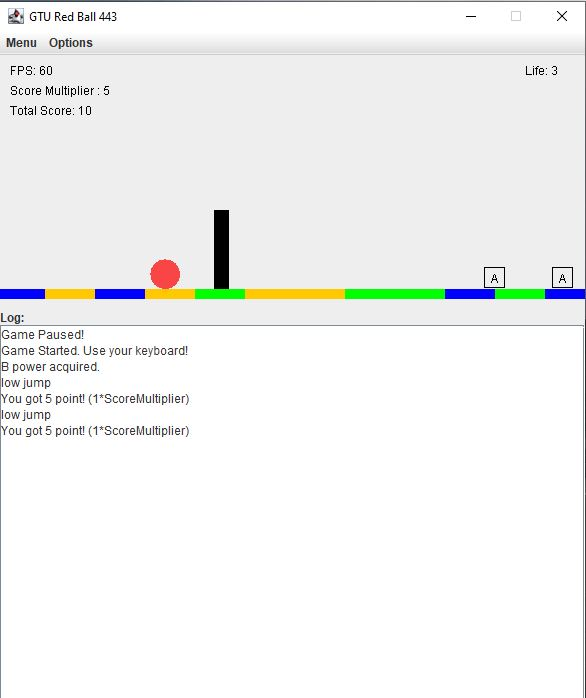
\includegraphics[width=7in, height=6in]{t1.JPG}
	\caption[Optional caption]{Picture from Game}
	\label{}
\end{figure}

\subsection{Design Patterns}
This game was implemented by using strategy and decorator design patterns.
\subsubsection{Strategy Design Pattern}
\begin{figure}[H]
    \centering
	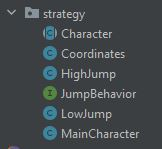
\includegraphics[width=3in, height=2in]{t2.JPG}
	\caption[Optional caption]{Classes in Strategy Design Pattern}
	\label{}
\end{figure}
Character is abstract class and JumpBehavior is an interface. 
\begin{figure}[H]
    \centering
	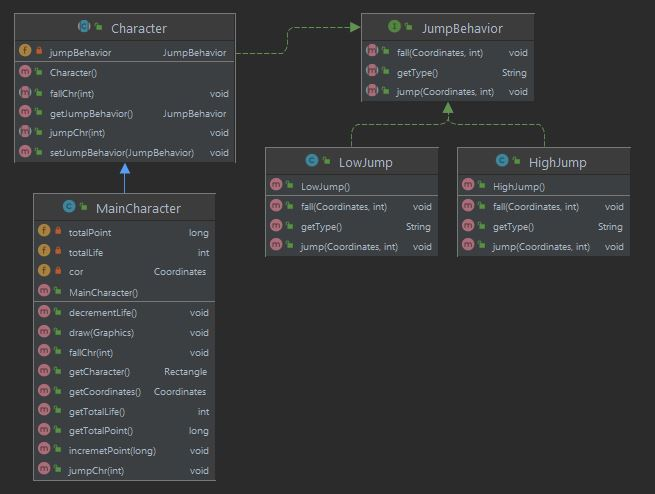
\includegraphics[width=7in, height=5in]{t3.JPG}
	\caption[Optional caption]{Simple Class Diagram for Strategy Design Pattern}
	\label{}
\end{figure}
\subsubsection{Decorator Design Pattern}
\begin{figure}[H]
    \centering
	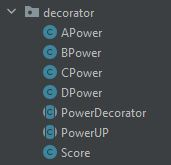
\includegraphics[width=3in, height=2in]{t4.JPG}
	\caption[Optional caption]{Classes in Decorator Design Pattern}
	\label{}
\end{figure}
PowerUP and PowerDecorator are abstract classes.
\begin{figure}[H]
    \centering
	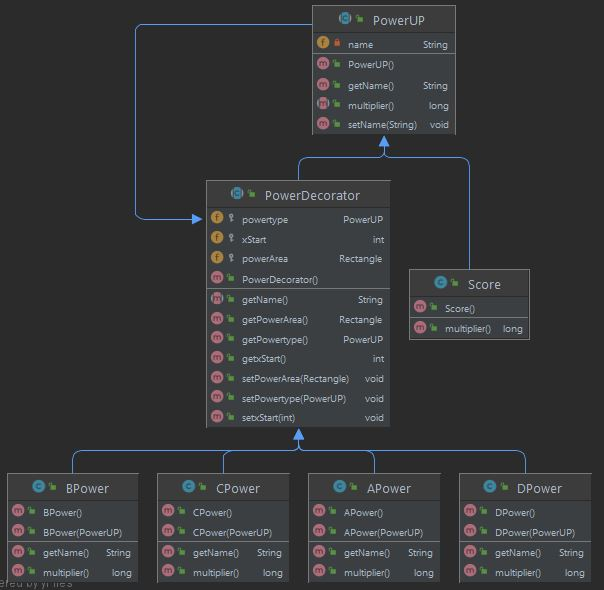
\includegraphics[width=7in, height=6in]{t5.JPG}
	\caption[Optional caption]{Simple Class Diagram for Decorator Design Pattern}
	\label{}
\end{figure}
\section{Class Diagrams}
In order to see class diagrams check class diagrams folder. 
\section{References that was used} 
\begin{itemize}
	\item Head First Design Patterns, 2nd Edition.
	\item Online sources to learn java gui.
	\item Eclipse editor to implement java gui.
	\item IntelliJ IDEA editor to create class diagrams.
\end{itemize}

   
\end{document}